%UNIT 1: QUALITATIVE AND GRAPHICAL APPROACHES
% Is first part of original 01.tex
%%%%%%%%%%%%%%%%%%%%%%%%%%%
%%%% Put the following at the top of each .tex file  %
\pagestyle{fancy}
\renewcommand{\theUnit}{3}
\ifthenelse{\isundefined{\UnitPageNumbers}}{}{\setcounter{page}{1}}
\rhead{Carlton and Devore Chapter \theUnit: Continuous Random Variables}
\lhead{Math 3382: Statistical Theory}
%\lhead{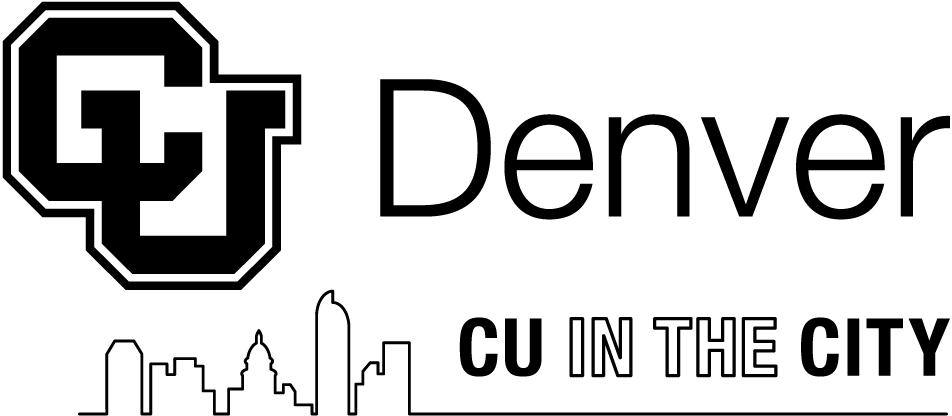
\includegraphics[width=1.25cm]{CUDenver-Logo.png}}
\rfoot{\mypage}
\cfoot{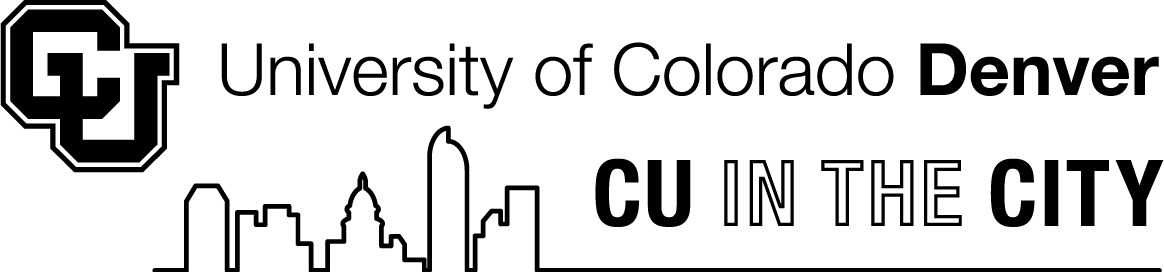
\includegraphics[width=2.25cm]{CUDenver-Logo-coverpage.png}}
\lfoot{Adam Spiegler}
\fancypagestyle{firstfooter}{\footskip = 50pt}
\renewcommand{\footrulewidth}{.4pt}
%%%%%%%%%%%%%%%%%%%%%%%%%%%
\vspace*{-20pt} \thispagestyle{firstfooter}

\pagebegin{Uniform Distributions}

\begin{tcolorbox}
Recall the \textbf{\colorb{uniform distribution}} of GPA's in problem \ref{gpa-uniform}. More generally, if a continuous random variable is uniformly distributed on the interval $\lbrack a , b \rbrack$, then
\bi
\ii The pdf is $\dsty f(x) = \left\{ \begin{array}{ll} \frac{1}{b-a}, & \hspace{12pt} a \leq x \leq b\\ 0, & \hspace{12pt} \mbox{otherwise} \end{array} \right.$.
\ii The cdf is
\[  F(x) = \left\{ \begin{array}{ll} 0, & \hspace{12pt} x<a \\ \frac{x-a}{b-a}, & \hspace{12pt} a \leq x \leq b \\ 1,  & \hspace{12pt}  x>b \end{array} \right.\]
\ii $E(X) = \frac{a+b}{2}$; $\Var(X) = \frac{(b-a)^2}{12}$; Median $=E(X) = \frac{a+b}{2}$.
\ei
\end{tcolorbox}

\pagebegin{Normal Distributions}

\begin{multicols}{2}
There are many cases where the data tends to be distributed symmetrically around a central value with no bias to the left or
right like this\footnote{Photograph by Peter Morenus in conjunction with Professor Linda Strausberg, of the University of Connecticut}:  %Subjects are University of Connecticut genetics students, females in white tops, males in dark tops}:

\columnbreak

\begin{center} 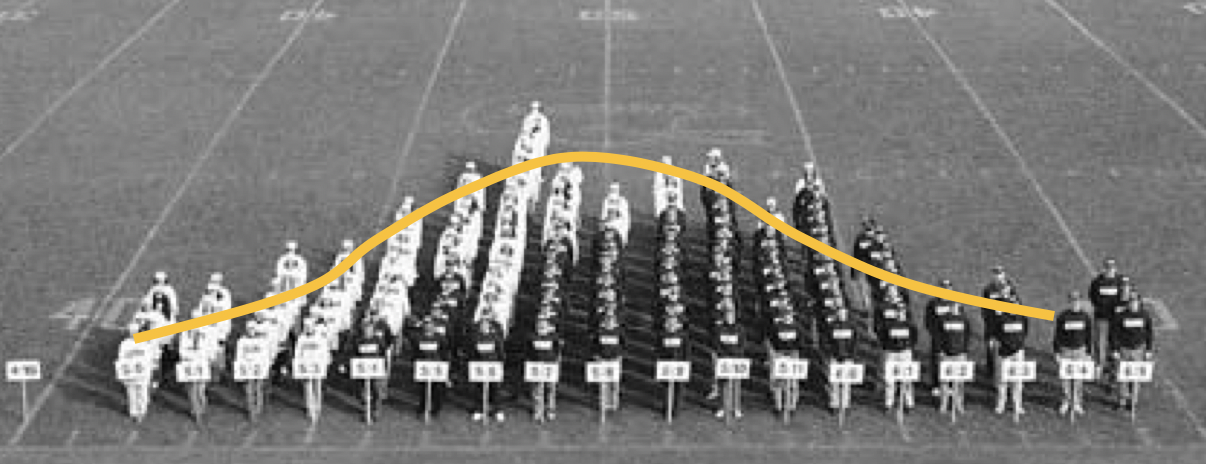
\includegraphics[width=3in]{07/07people.png}\end{center}

\end{multicols}

Normal distributions arise in many settings: Heights of people, size of items produced by machines, and most importantly in statistics data sets resulting from many independent random events. \medskip

\begin{tcolorbox}

The shape of a \textbf{\colorb{normal distribution}} are determined by two parameters:
\bi
\ii The \colorr{mean, $\mu$}, is center of the distribution.
\ii The \colorr{standard deviation, $\sigma$}, tells us how wide the distribution is.
\ii If $X$ is normally distributed with mean $\mu$ and standard deviation $\sigma$, we write \colorr{$\mathbf{X \sim N(\mu, \sigma)}$}.
\ei

\end{tcolorbox}

\begin{tabular}{|c|c|}
\hline
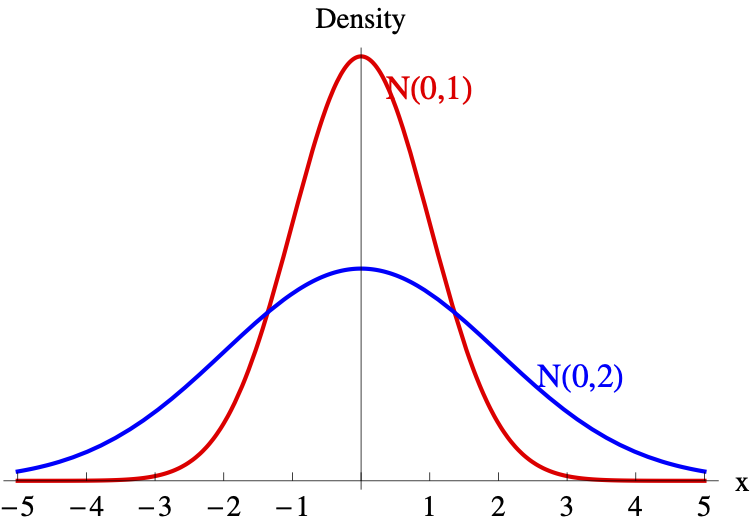
\includegraphics[width=0.35\tw]{07/07normal-width.pdf} & 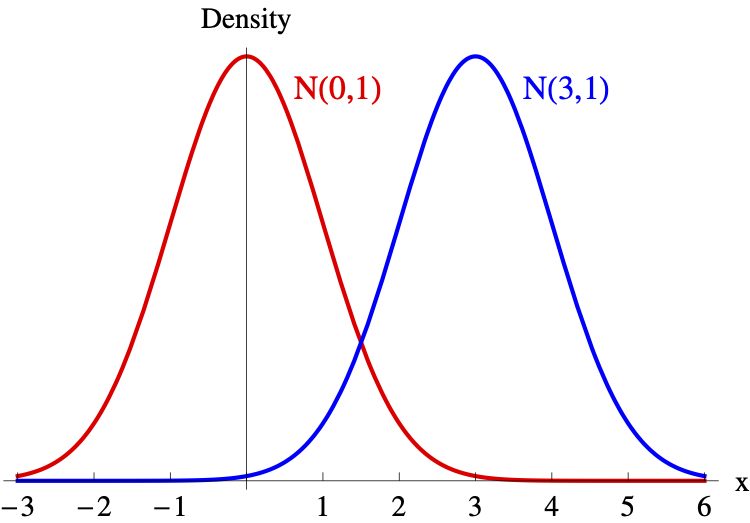
\includegraphics[width=0.35\tw]{07/07normal-center.pdf}\\
\hline
{\scriptsize Increasing the standard deviation makes the curve wider.} &
{\scriptsize Increasing the mean shifts the center of the graph.} \\
\hline
\end{tabular}


\clearpage

\pagebegin{Using the Empirical Rule}

\begin{tcolorbox}
\begin{multicols}{2}
The \textbf{\colorb{empirical rule}} for normal distributions:
\bi
\ii 68\% of all values fall within one standard deviation (both above and below) from the mean, and 
\ii 95\% of all values fall within two standard deviations of the mean.
\ii 99.7\% of all values fall within three standard deviations of the mean.
\ei

\columnbreak

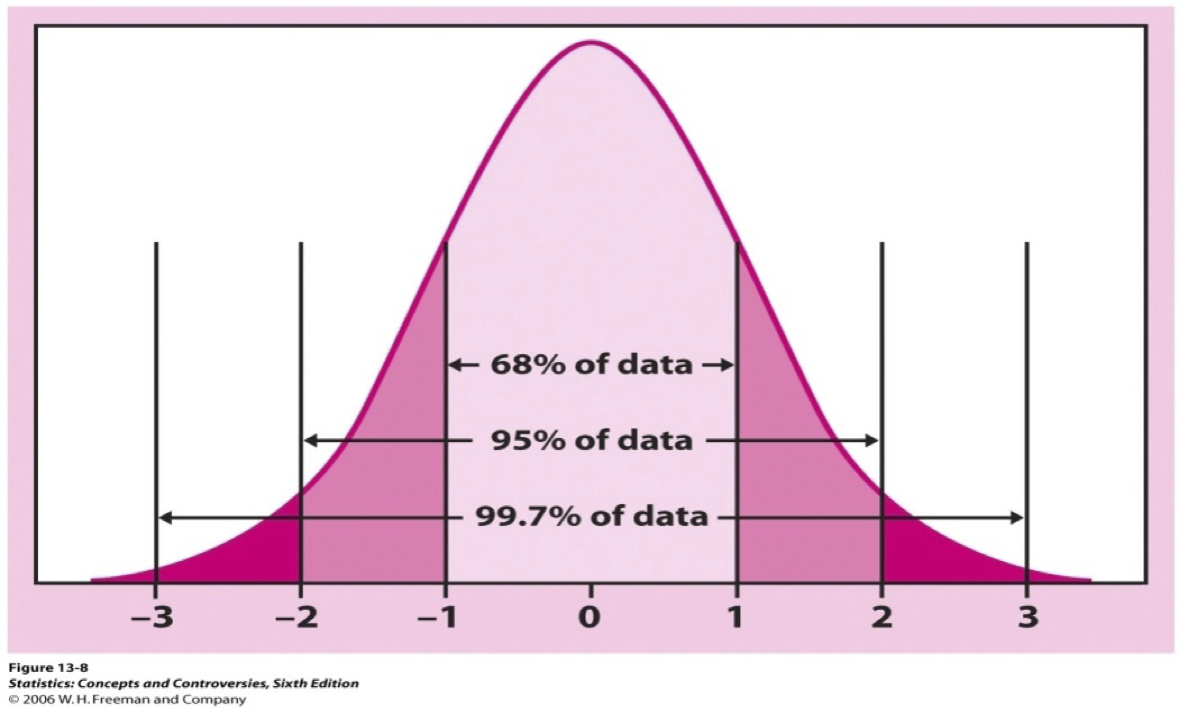
\includegraphics[width=0.45\tw]{07/07empirical.pdf}

\end{multicols}
\end{tcolorbox}

\bb[resume]
\ii ``Last night, Israel became the first country ever to pass legislation banning the use of ‘underweight’ models in local ads and publications. The new law employs an interesting tactic: Models must prove that their Body Mass Index (BMI) is higher than the World Health Organization's indication of malnourishment (a BMI of 18.5) by producing an up-to-date medical report — no older than three months — at all shoots to be used in the Israeli market.'' \footnote{Israel Passes Law Requiring Models to Show Health Records and Meet Weight Standards”, New York Magazine by Charlotte Cowles on April 20, 2012}\label{BMI}

\bi
\ii Let $X$ denote the BMI of adult men in Israel. We know that $X \sim N(26,4)$.
\ii Let $Y$ denote the BMI of adult women in Israel. We know that $Y \sim N(26.5,4.5)$.
\ei

\bb
\ii What proportion of the men in Israel have BMI between 26 and 30? \vfill
\ii What proportion of the women in Israel have BMI between 22 and 35.5? \vfill
\ii How many standard deviations from the mean is a male BMI of 21? \vfill
\ee
\ee

\clearpage

\pagebegin{$Z$-Scores and the Standard Normal Distribution}

\begin{tcolorbox}
\begin{definition}\label{def:zscore}
The number of standard deviations a given data value is from the mean is called the
\textbf{\colorb{z-score}} for the value and is calculated using the formula
\[ z = \frac{x-\mu}{\sigma}.\]
\end{definition}
\end{tcolorbox}

For example, the $z$-score of a male with a BMI 21 is $z=\frac{21-26}{4} = -1.25$.

\begin{center}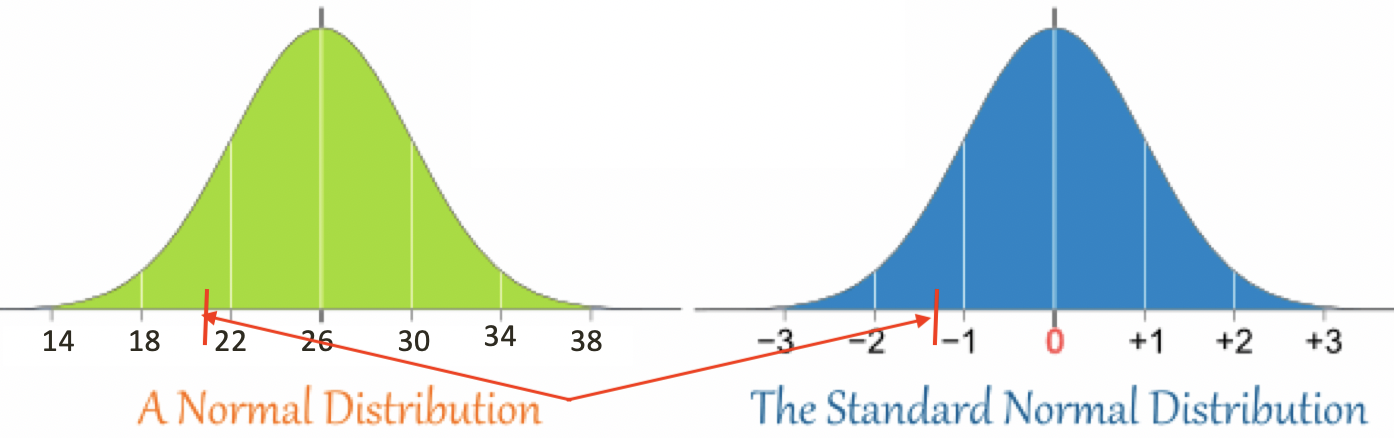
\includegraphics[width=0.75\tw]{07/07normal-stand.png} \end{center}

When you compute the z-score, you are \textbf{\colorr{“standardizing”}} your data.  You describe values in terms of how many standard deviations from they are from the mean. Comparing areas, we see that \\ $P(X<21) = P(Z<-1.25)$.


\bb[resume]
\ii BMI distribution is approximately normal. In Israel, women have mean BMI of $26.5$ with a standard deviation $4.5$.
What proportion of the women in Israel are legally “underweight” (BMI $< 18.5$)?

\bb
\ii Calculate the $z$-score of a Israeli woman with a BMI of $18.5$. \vfill
\ii Interpret the meaning of the value  in part (a), and give an estimate for the proportion of women in Israel who are legally underweight. \vfill
\ee
\ee

\begin{tcolorbox}
The probability density function for normal distribution (or Gaussian) $X \sim N(\mu,\sigma)$ is given by the formula

\[ f(x) = \frac{1}{\sigma\sqrt{2\pi}} e^{-\frac{1}{2} \left( \frac{x-\mu}{\sigma} \right)^2}\]

To find the probability that a woman has a BMI less than $18.5$, we could try to evaluate

\[ P(\mbox{BMI} < 18.5) = \int_{0}^{18.5} \frac{1}{4.5\sqrt{2\pi}} e^{-\frac{1}{2} \left( \frac{x-26.5}{4.5} \right)^2} \, dx\]

YIKES, good luck with that! So we need to find other methods.
\end{tcolorbox}

\clearpage

\pagebegin{Calculating Areas Under Normal Distributions}


\bb[resume]
\ii What proportion of women in Israel are below the $18.5$ BMI limit?
\ee

\vfill

Using the standard normal distribution table:

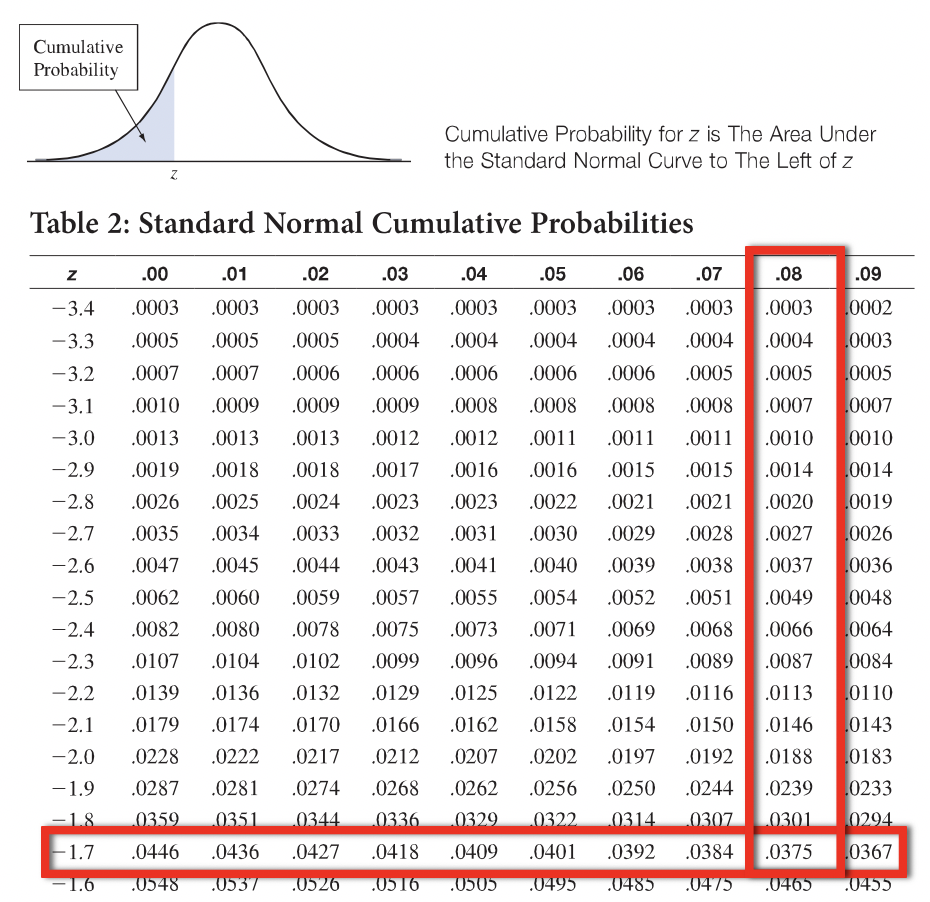
\includegraphics[width=0.75\tw]{07/07table.png} \medskip

\begin{tcolorbox}
Using R:
\bi
\ii pnorm($x$, $\mu$, $\sigma$)$=P(X<x)$ gives the area to the left of $x$ under $N(\mu,\sigma)$.
\ii pnorm($x$, $\mu$,  $\sigma$, lower.tail=FALSE)$=P(X>x)$ gives the area to the right of $x$ under $N(\mu,\sigma)$.
\ei \medskip

Or you can find the $z$-score and use the standard normal distribution in R as well:
\bi
\ii pnorm($z$, 0,1)$=P(Z<z)$ gives the area to the left of $x$ under $N(0,1)$.
\ii pnorm($z$, 0,  1, lower.tail=FALSE)$=P(Z>z)$ gives the area to the right of $x$ under $N(0,1)$.
\ei
\end{tcolorbox}

\clearpage

\pagebegin{Practice: IQ Scores}

\bb[resume]
\ii Intelligence quotient (IQ) scores are normally distributed. The mean IQ score is 100 points and the standard deviation is 16 points.

\bb
\ii What proportion of people have an IQ score above 116? \vfill
\ii Marilyn vos Savant has been known to have the highest recorded IQ in the world.  The $z$-score of her test result is $z=5.4$.  What is her IQ score? \vfill
\ii What proportion of people have an IQ score between 75 and 100? \vfill
\ii What is the 90th percentile for IQ? In other words, find the IQ score such that 90\% of the people score less than that score. \vfill
\ee
\ee

\bb[resume]
\ii Let $X$ denote the time (in minutes) spent waiting for the next light-rail to arrive at Union Station. Sketch a possible graph for the probability distribution function of $X$. Explain how you determined the shape of your graph. \vfill
\ee

\clearpage

\pagebegin{Exponential Distribution: Section 3.4}


\begin{tcolorbox}
\bi
\ii Uniform distributions model situations in which each outcome has an equally likely chance to occur.
\ii Most people are average height, but there are approximately an equal number of shorter and taller people. This can be modeled using a normal distribution.
\ii Most of the time, you do not need to wait very long for the next light rail. But sometimes, though rarely,  you do get 
stuck waiting a longer amount of time.
\ii The waiting time for the light rail has properties that can be modeled using an \textbf{\colorb{exponential distribution}}.
\ei

If a continuous random variable $X$ is \textbf{\colorb{exponentially distributed}}, the shape of its pdf depends on one parameter, $\lambda = \frac{1}{\mu}$ where $\mu$ denotes the average value of $X$. We write $X \sim Exp(\lambda)$.

\bi
\ii The pdf is $\dsty f(x) = \lambda e^{-\lambda x}$ for $x >0$ where $\lambda = \frac{1}{\mu}$.
\ii $E(X) = \frac{1}{\lambda}=\mu$ and $\Var(X) = \frac{1}{\lambda^2} = \mu^2$.
\ei
\end{tcolorbox}

\pagebegin{Practice: 911 Call Center}

\bb[resume]
\ii At a 911 call center, calls come in at an average rate of one call every two minutes. Let $X$ denote the time that elapses from one call to the next, and assume $X$ has an exponential distribution.

\bb
\ii Give a formula and sketch the graph of the pdf $f$.  \vfill
\ii Find the probability that after a call is received, it takes more than three minutes for the next call to occur. Illustrate this value on your graph.  \vfill

\clearpage


\ii Find a formula for the cdf, $F$.  \vfill
\ii Find a formula for the inverse of the cdf, $F^{-1}$.  \vfill
\ii Ninety-percent of all calls occur within how many minutes of the previous call? Hint: Use your previous answer.  \vfill
\ii Suppose that two minutes have elapsed since the last call. Find the probability that the next call will occur within the next minute.  \vfill
%\ii Find the probability that less than 20 calls occur within an hour.
\ee
\ee



%During the years 1998 - 2012, a total of 29 earthquakes of magnitude greater than $6.5$ have occurred in Papua New Guinea. Assume that the time spent waiting between earthquakes is exponential.

%\bb
%\ii What is the probability that the next earthquake occurs within the next three months?
%\ii Given that six months has passed without an earthquake in Papua New Guinea, what is the probability that the
%next three months will be free of earthquakes?
%\ii What is the probability of zero earthquakes occurring in 2016?
%\ii What is the probability that at least two earthquakes will occur in 2016?
%\ee
